\documentclass{article}

\usepackage[spanish]{babel}
\usepackage[numbers,sort&compress]{natbib}
\usepackage{graphicx}
\usepackage{url}
\usepackage{amsmath}
\usepackage{hyperref}
\usepackage[top=30mm, bottom=40mm, left=15mm, right=15mm]{geometry}
\usepackage{listings}
\usepackage{subfig}
\usepackage{color}

\setlength{\parskip}{2mm}
\setlength{\parindent}{0pt}
\definecolor{dkgreen}{rgb}{0,0.6,0}
\definecolor{gray}{rgb}{0.3,0.3,0.3}
\definecolor{orange}{rgb}{0.8,0.4,0}
\definecolor{mostaza}{rgb}{0.9,0.8,0.1}

\lstset{ %
  language=R,                     % the language of the code
  basicstyle=\footnotesize,       % the size of the fonts that are used for the code
  numbers=left,                   % where to put the line-numbers
  numberstyle=\tiny\color{gray},  % the style that is used for the line-numbers
  stepnumber=1,                   % the step between two line-numbers. If it's 1, each line
                                  % will be numbered
  numbersep=5pt,                  % how far the line-numbers are from the code
  backgroundcolor=\color{white},  % choose the background color. You must add \usepackage{color}
  showspaces=false,               % show spaces adding particular underscores
  showstringspaces=false,         % underline spaces within strings
  showtabs=false,                 % show tabs within strings adding particular underscores
  frame=single,                   % adds a frame around the code
  rulecolor=\color{black},        % if not set, the frame-color may be changed on line-breaks within not-black text (e.g. commens (green here))
  tabsize=2,                      % sets default tabsize to 2 spaces
  captionpos=b,                   % sets the caption-position to bottom
  breaklines=true,                % sets automatic line breaking
  breakatwhitespace=false,        % sets if automatic breaks should only happen at whitespace
  title=\lstname,                 % show the filename of files included with \lstinputlisting;
                                  % also try caption instead of title
  keywordstyle=\color{orange},      % keyword style
  commentstyle=\color{dkgreen},   % comment style
  stringstyle=\color{mostaza},      % string literal style
  escapeinside={\%*}{*)},         % if you want to add a comment within your code
  morekeywords={*,...}            % if you want to add more keywords to the set
} 

\author{Marco Antonio Guajardo Vigil 2095}
\title{\textbf{Diagramas de Voronoi} \\ Simulaci\'on de sistemas}
\date{\today}

\begin{document}

\maketitle

\section{Introducci\'on}
Los \textit{diagramas de Voronoi} tienen importancia en las matem\'aticas puras y en las ciencias aplicadas como por ejemplo la ciencia de los materiales. Se toma de un espacio bidimensional una zona con medidas conocidas que contienen \textit{k} puntos de semilla $P_i$, los cuales son representados por sus coordenadas ($X_i, Y_i$). Se busca dividir esa zona en regiones llamadas \textit{celdas de Voronoi} de tal forma que todos los puntos que pertenecen a la regi\'on de $P_i$ est\'en m\'as cerca de esa semilla que a cualquier otra \cite{SatuP4}.

Para esta pr\'actica se utiliza el \textbf{diagrama de Voronoi} para crear un modelo matem\'atico cont\'inuo, es decir, las coordenadas son n\'umeros reales. Se representa la zona por una matriz \textbf{n x n} y las coordenadas son n\'umeros enteros en \textbf{\textit{[1, n]}}.
Se coloca uniformemente al azar las \textbf{\textit{k}} semillas, representadas por los n\'umeros \textbf{\textit{1}} a \textbf{\textit{k}} dentro de la matriz, procurando que ocupen una posici\'on distinta, como se muestra en la figura \ref{fig:Zona}.

\begin{figure}[h!]
\centering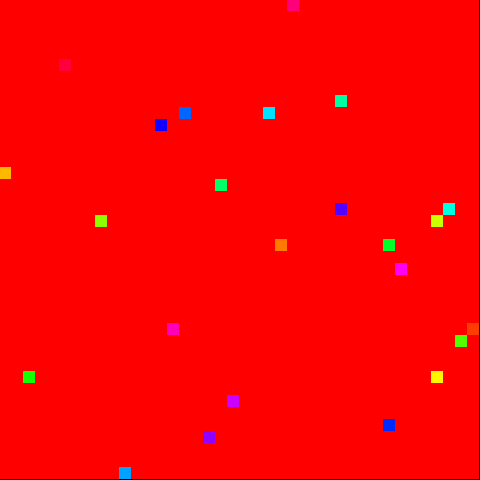
\includegraphics[width=80mm]{p4s.png}
\caption{Representaci\'on de una zona de Voronoi de 40 x 40, con 24 semillas.}
\label{fig:Zona}
\end{figure}

\newpage

\section{Implementaci\'on de R}
Para la elaboraci\'on de este experimento, se hace uso de un software libre para computaci\'on estad\'istica y gr\'aficos llamado \citet{R}, el cual nos permite realizar los c\'alculos necesarios para dicho experimento. Con \'el, se pueden controlar los datos estad\'isticos que se ocupan para dar seguimiento con la pr\'actica, se necesita graficarlos para as\'i poder compararlos mejor, ya que se maneja una cantidad de datos considerable y trabajaremos con ellos en forma estad\'istica, por lo tanto, se recomienda el uso de este software ya que ayuda a paralelizar las acciones que sean necesarias, as\'i se ahorra tiempo, haci\'endolas simult\'aneamente.

\section{Experimentaci\'on}

Para llevar a cabo este experimento, se realiza una variaci\'on de los parametros \textbf{\textit{n}} (dimensi\'on de la zona) y \textbf{\textit{k}} (n\'umero de semillas), se hacen 20 r\'eplicas para cada variaci\'on de \textbf{\textit{k}} y \textbf{\textit{n}}. Se utiliza otro m\'etodo para obtener las distancias de las grietas propagadas usando \textit{Manhattan}, esto es debido con el fin de detectar grietas peligrosas en base de la distancia m\'as alejada que llego a estar de un borde cercano de la zona. Se realiz\'o un resumen de los datos recaudados del experimento y fueron guardados en un \textit{data.frame} llamado \textbf{datos}.

\begin{lstlisting}[language=R]
N <-  c(15,30,45,60)
K <- c(12,24,36,48)
datos <- data.frame()
Largo <- c()
Manhattan <- FALSE
replicas <- 20
\end{lstlisting}

Para controlar el manejo de las distancias a usar, siendo las celdas recorridas por la grieta o distancia \textit{Manhattan}, se utiliza el siguiente c\'odigo, el cual es controlado por una variable llamada \textbf{Manhattan} cuyo valor booleano viene por default como \textbf{FALSE}, para as\'i, encontrar los largos por la distancia de las celdas recorridas, en caso de que este obtenga un valor \textbf{TRUE} encontrara las distancias m\'aximas mediante \textit{Manhattan}:

\begin{lstlisting}[language=R]
if (Manhattan){
    return(abs(i[1] - xg) + abs(i[2] - yg))
} else {
    return(largo)
  }
}
\end{lstlisting}

\newpage

La acumulaci\'on de los datos en el data frame se realiza mediante la finalizaci\'on de cada r\'eplica de modo que se sit\'uan como se muestra en el siguiente parte del c\'odigo.

\begin{lstlisting}[language=R]
for(n in N){
    for(k in K){
        ...
        suppressMessages(library(doParallel))
        registerDoParallel(makeCluster(detectCores() - 1))
        largos <- foreach(r = 1:replicas, .combine=c) %dopar% propaga(r)
        stopImplicitCluster()
        sum <- c(n, k, summary(largos))
        datos <- rbind(datos, sum)
        Largo <- c(Largo, largos)
        colnames(datos) <- c("n", "k", "Min", "Q1", "Median", "Mean", "Q3", "Max")
    }
}
\end{lstlisting}

Los resultados obtenidos se grafican con ayuda de \textbf{ggplot} en forma de \textit{boxplot}:

\begin{lstlisting}[language=R]
 g <- ggplot(datos, aes(x = as.factor(k), ymin = Min, lower = Q1, middle = Mean, upper = Q3, ymax = Max, fill = as.factor(k)))
 g <- g + geom_boxplot(stat = "identity") + theme_gray(base_size = 14) + labs(x = "Tama\u{F1}o de la zona (n)", y = "Largo de la grieta")
 g <- g + scale_fill_brewer(palette= "BuPu") + facet_grid(~n) + theme(legend.position="none")
 g
 ggsave("LargoDeGrieta.png")
\end{lstlisting}

\newpage

\section{Resultados}

\subsection{Recorrido de celdas}

\begin{figure}[h!]
\centering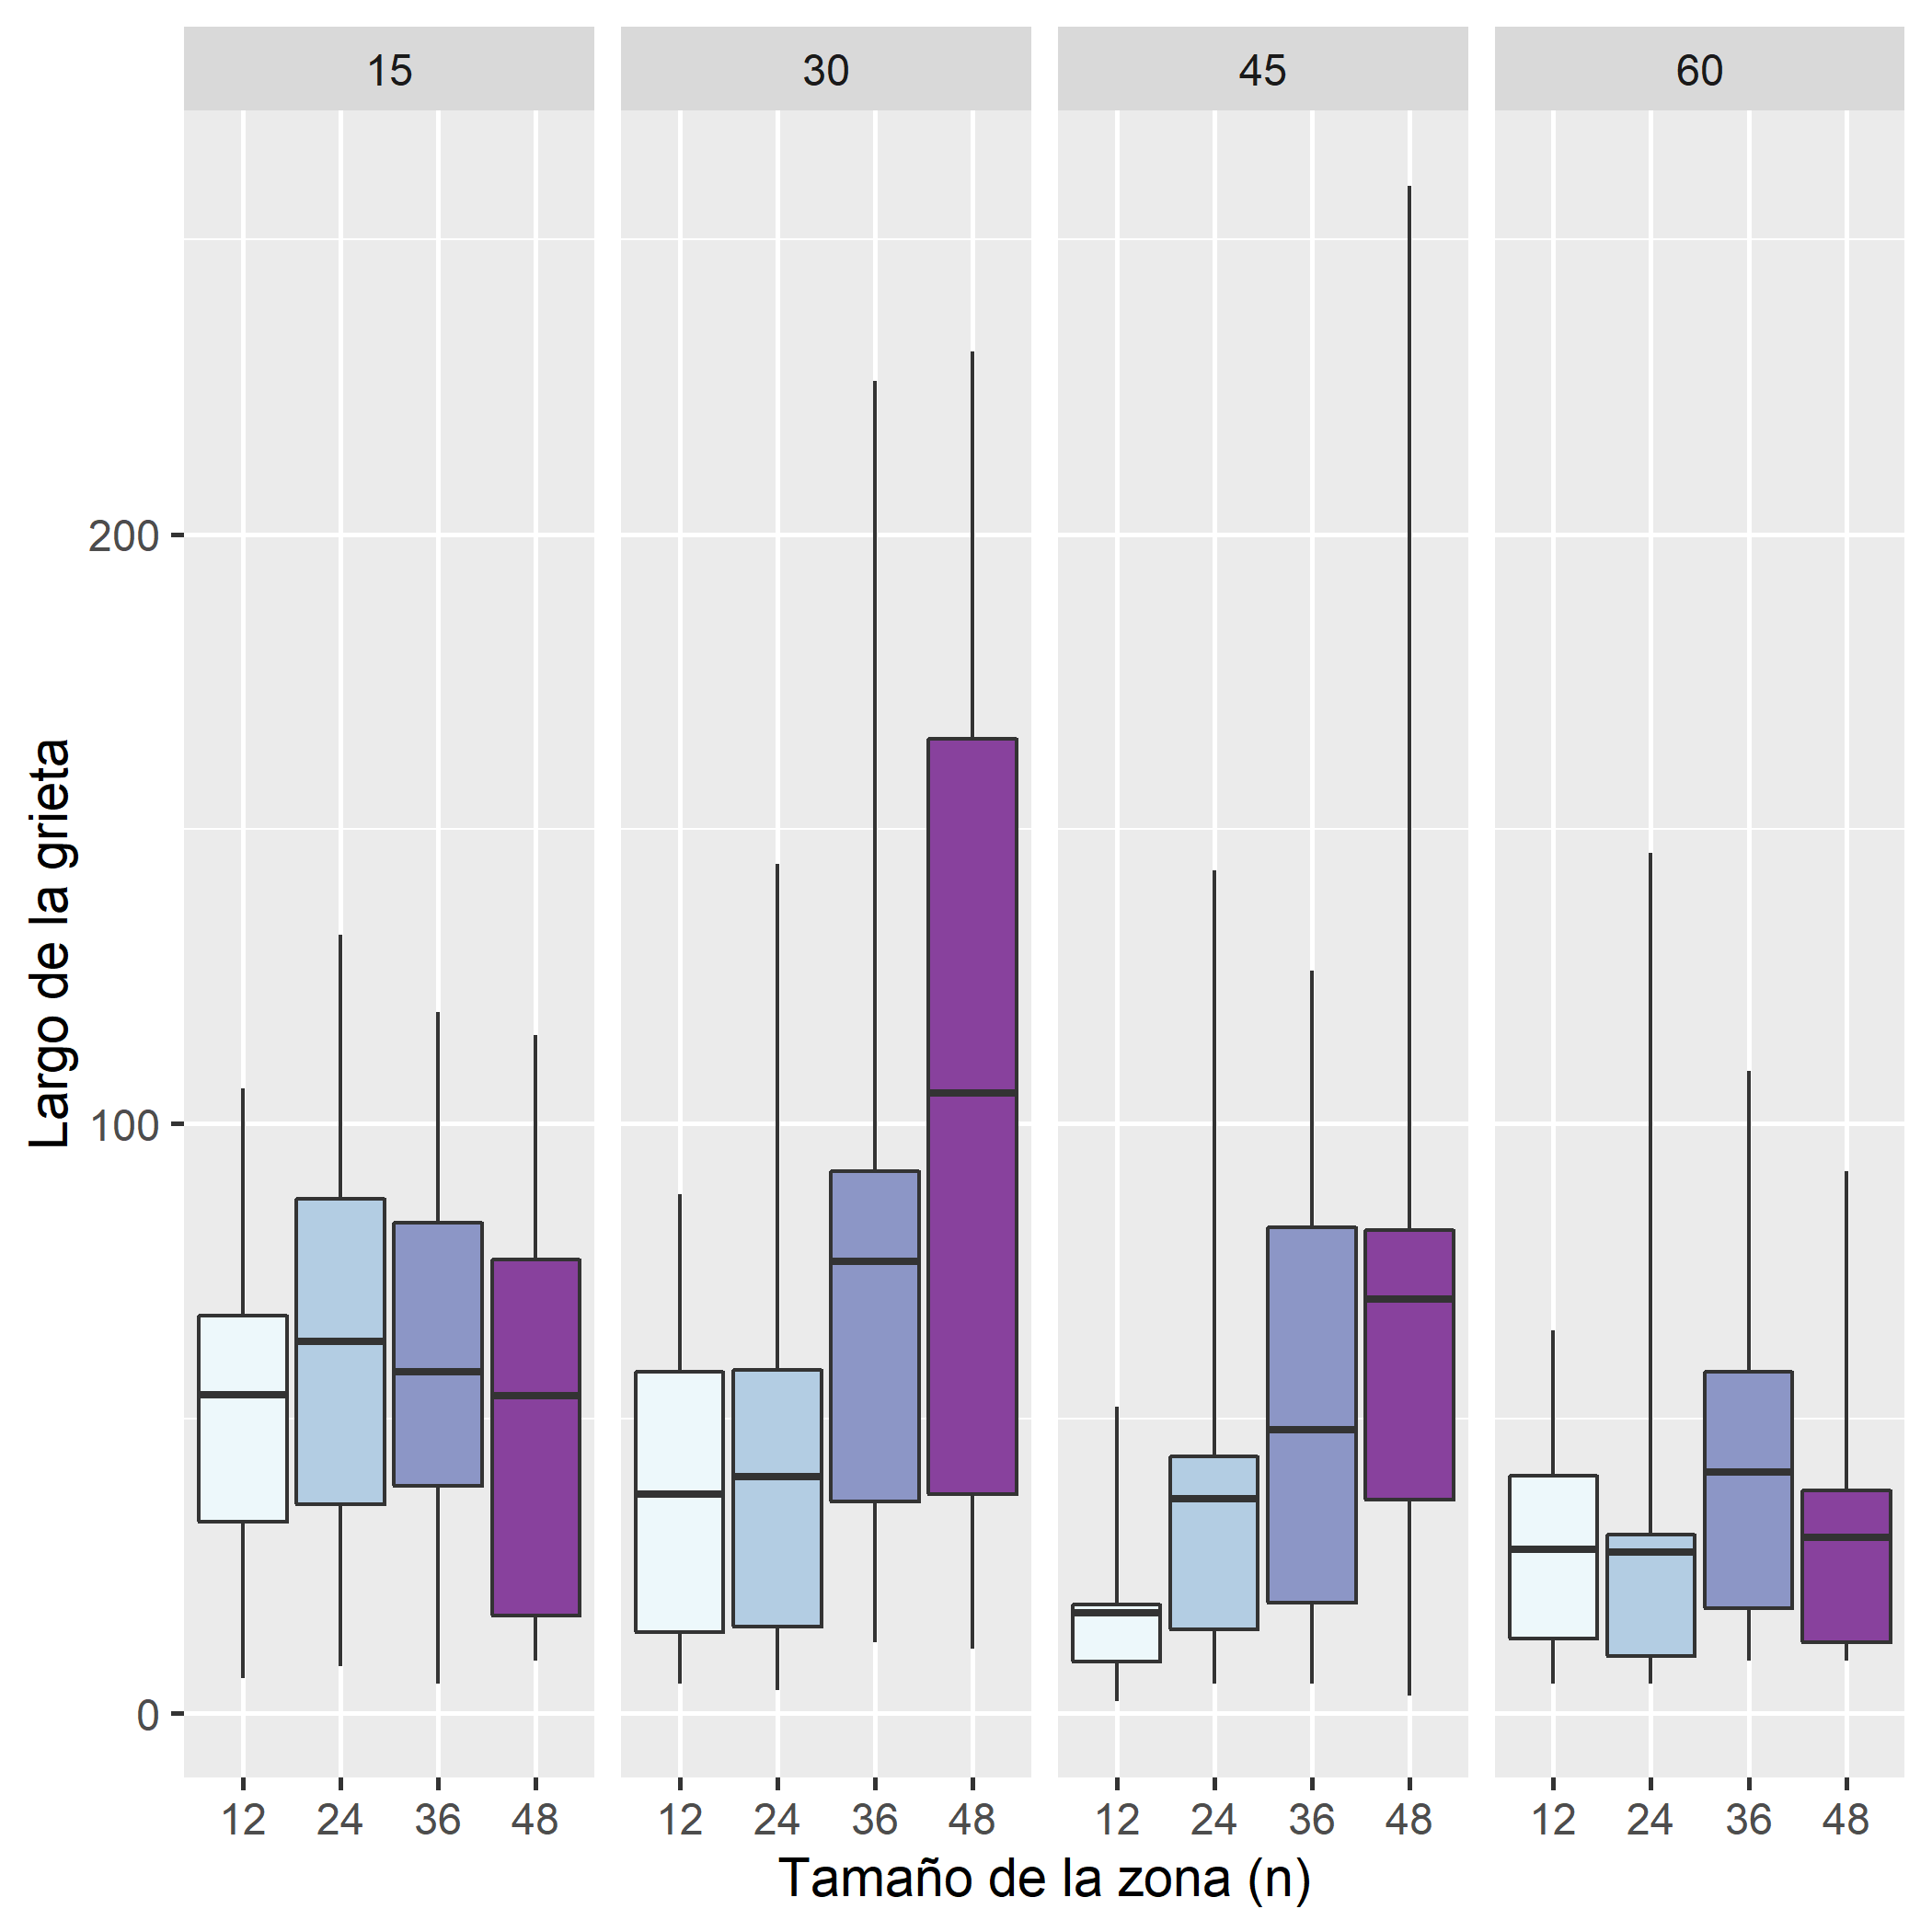
\includegraphics[width=120mm]{LargoDeGrieta.png}
\caption{Resultados de variaciones por el recorrido de celdas.}
\label{fig:Grieta}
\end{figure}

Con la distancia m\'axima por el recorrido de celdas, mostradas en la figura \ref{fig:Grieta}, es notable que las variaciones tanto de \textbf{k} como \textbf{n} afectan en la distancia que llega a recorrer la grieta, cuando \textit{k} = 48 y \textit{n} = 30, llega a mostrar las distancias m\'as largas, con una media de 110 aproximadamente. Cuando \textbf{k} es mayor a \textbf{n}, las distancias son mayores.

\newpage

\subsection{Recorrido usando Manhattan}

\begin{figure}[h!]
\centering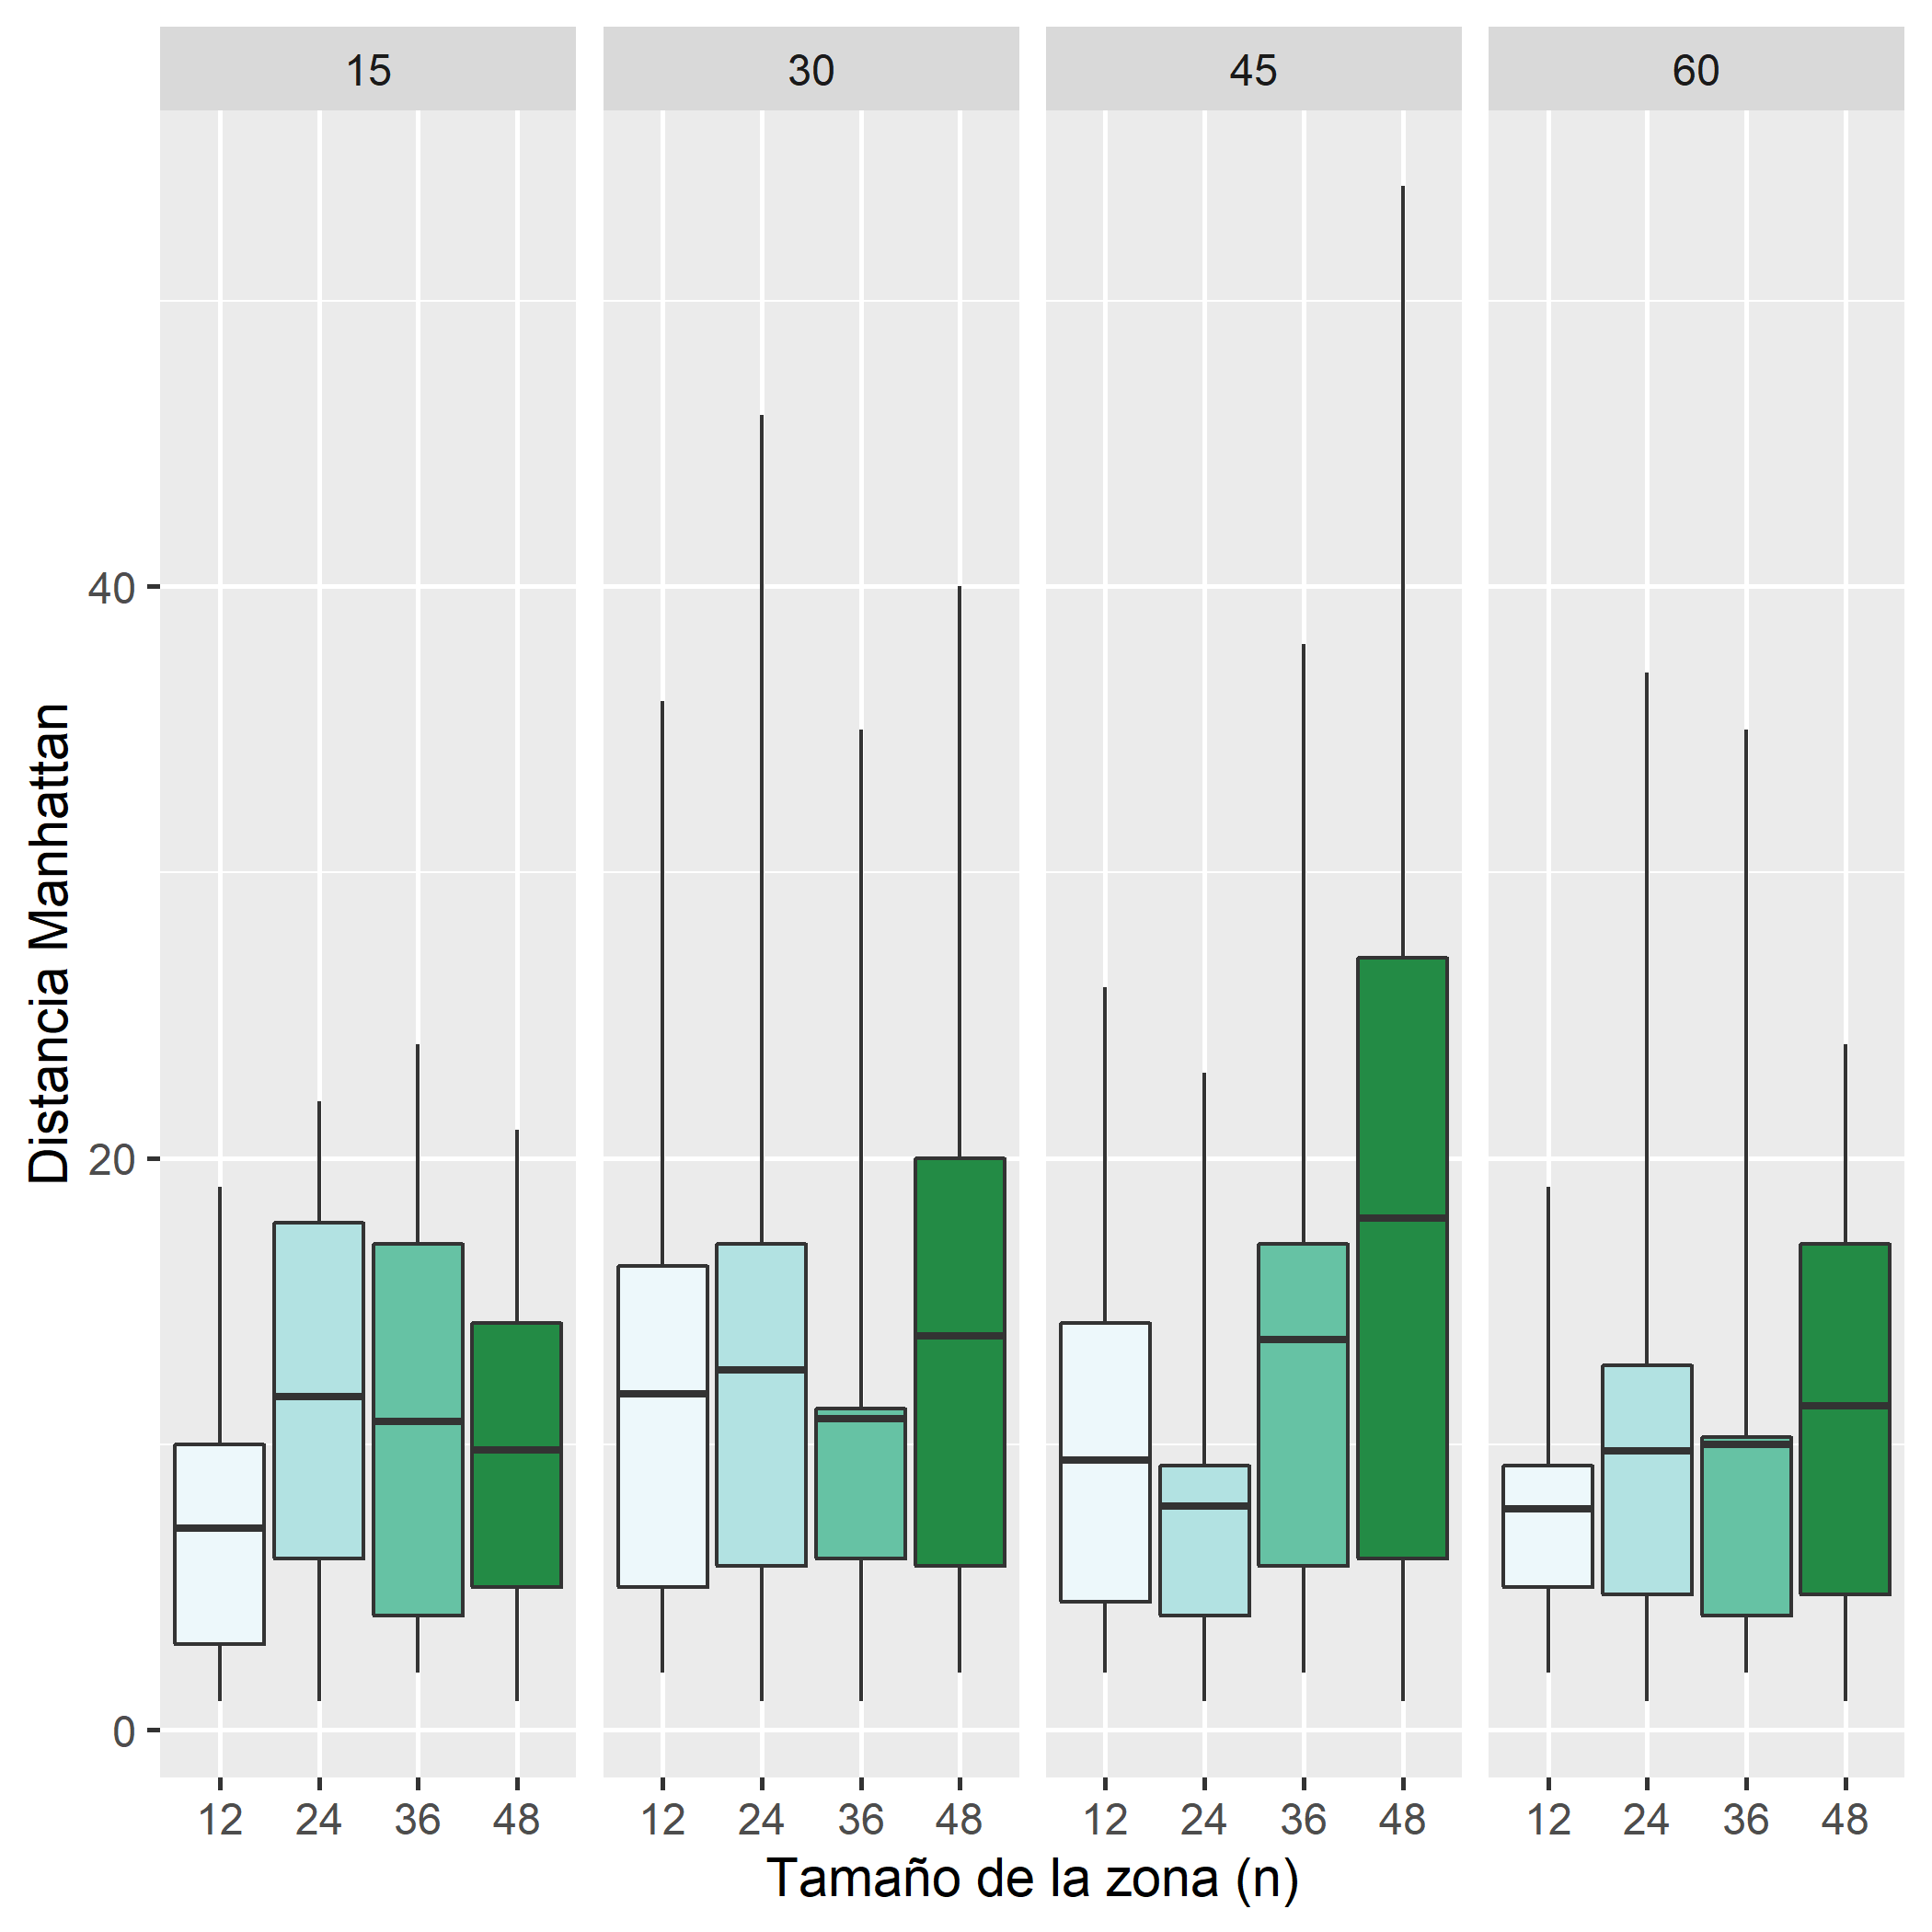
\includegraphics[width=120mm]{Manhattan.png}
\caption{Resultados de variaciones por el recorrido Manhattan.}
\label{fig:Manhattan}
\end{figure}

En la figura \ref{fig:Manhattan}, la distancia de mayor de las grietas baja considerablemente, ya que, con el recorrido por celdas, esta distancia suele ser mucho mayor sobrepasando los doscientos, en cambio, aqu\'i llegan a un m\'aximo de cincuenta. La distancias largas en este recorrido son m\'as realistas que con el recorrido de celdas, por lo tanto, cuando \textbf{k} y \textbf{n} aumentan, estas grietas se vuelven cada vez mas peligrosas, en especial con el n\'umero de semillas, como se observa en la ultima variaci\'on de \textbf{n}.

\section{Conclusi\'on}

La grieta tiene m\'as oportunidad de propagarse cuando hay una gran cantidad de semillas esparcidas en la zona, aunque, si la zona es mucho mas grande, la grieta puede empezar a batallar cada vez m\'as en propagarse, puesto que ahora tiene mayor distancia que recorrer.

\bibliographystyle{plainnat}
\bibliography{Bibliografias}
\end{document}